%"###############################################
%
% Classification supervisée
%
%###############################################

% VPPBS: variables post-op à 12 mois
%
%###############################################

\subsubsection{VPPBS: IPSS à 12 mois}

Nous appliquons la même méthode que précédemment sur les données VPPBS.
Nous obtenons un arbre de régression sur la seule variable PSA (figure~\ref{fig-vppbs-regtree-ipss12}) qui indique sur chaque feuille la probabilité des valeurs respectives d'IPSS à 12 mois: 0/1/2/3/4/5/13, constatées sur l'ensemble d'apprentissage.

\begin{figure}[H]
\centering
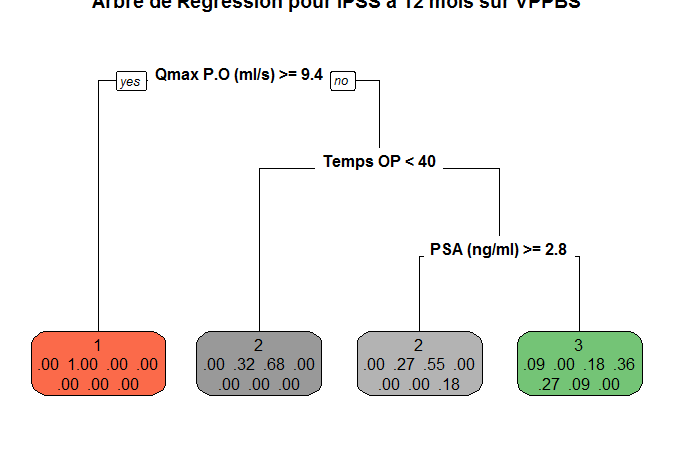
\includegraphics[width=0.75\textwidth]{../Fig/VPPBS/vppbs-regtree-ipss12.png}
\caption{VPPBS: Arbre de régression pour IPSS à 12 mois}
\label{fig-vppbs-regtree-ipss12}
\end{figure}

La figure~\ref{fig-vppbs-regtree-predict-ipss12} représente plus visuellement les probabilités prédites par cet arbre de régression pour l'ensemble de validation. On s'aperçoit que la plus forte probabilité qui ressort est quasi systématiquement
IPSS==2, alors que cette valeur correspond à la valeur de référence pour le patient 40 seulement. Cela est dû au tirage aléatoire qui a suréchantillonné dans l'ensemble d'apprentissage les patients pour lesquels la valeur IPSS à 12 mois vaut 2, et sous échantillonné les patients pour lesquels la valeur IPSS à 12 mois vaut 3,4,5 ou 13.

Répéter la génération d'arbre de régression pour construire une forêt permettrait de
minimiser ce risque d'erreur. 

\begin{figure}[H]
\centering
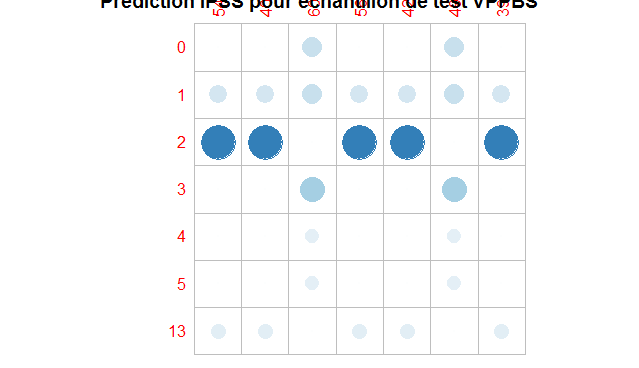
\includegraphics[width=0.75\textwidth]{../Fig/VPPBS/vppbs-regtree-predict-ipss12.png}
\caption{VPPBS: Prévision pour IPSS à 12 mois}
\label{fig-vppbs-regtree-predict-ipss12}
\end{figure}

\subsubsection{VPPBS: QoL à 12 mois}

On retrouve la variable PSA dans cet arbre de régression pour la QoL à 12 mois
qui infère des probabilités pour les valeurs respectives 0/1/3/5 (Cf. figure~\ref{fig-vppbs-regtree-qol12}. Le tirage aléatoire a ici exclus la valeur 2
(patient 60 uniquement) de l'ensemble d'apprentissage. La validation pour cette
valeur sera donc biaisée (Cf. figure~\ref{fig-vapor-regtree-predict-qol12})).

Répéter la génération d'arbre de régression pour construire une forêt permettrait de
minimiser ce risque d'erreur. 

\begin{figure}[H]
\centering
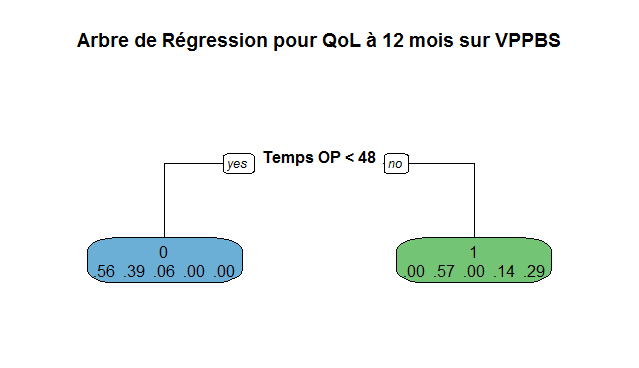
\includegraphics[width=0.75\textwidth]{../Fig/VPPBS/vppbs-regtree-qol12.png}
\caption{VPPBS: Arbre de régression pour QoL à 12 mois}
\label{fig-vppbs-regtree-qol12}
\end{figure}

\begin{figure}[H]
\centering
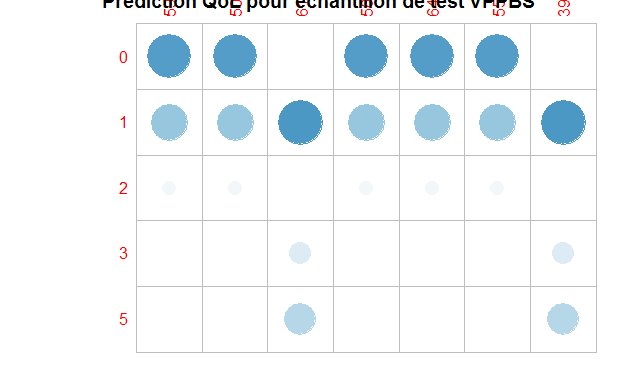
\includegraphics[width=0.75\textwidth]{../Fig/VPPBS/vppbs-regtree-predict-qol12.png}
\caption{VPPBS: Prévision pour QoL à 12 mois}
\label{fig-vppbs-regtree-predict-qol12}
\end{figure}


\subsubsection{VPPBS: Qmax à 12 mois}

L'arbre de régression obtenu pour la variable Qmax à 12 mois (colonne Qmax (ml/s)\_\_3) met en oeuvre une seule variable (Cf. figure~\ref{fig-vppbs-regtree-qmax12}). Les feuilles de l'arbre représentent, en première ligne, la valeur approximative pour Qmax à 12 mois. La ligne suivante indique le nombre de patients de l'échantillon d'apprentissage correspondant à cette feuille. 

\begin{figure}[H]
\centering
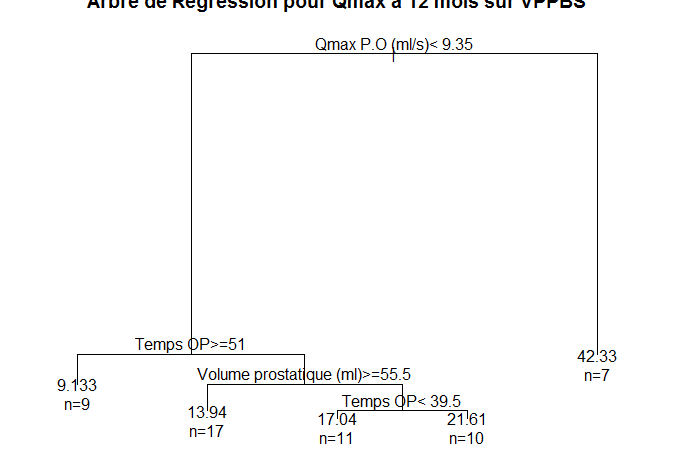
\includegraphics[width=0.75\textwidth]{../Fig/VPPBS/vppbs-regtree-qmax12.png}
\caption{VPPBS: Arbre de régression pour Qmax à 12 mois}
\label{fig-vppbs-regtree-qmax12}
\end{figure}

Pour évaluer l'arbre de régression, nous utiliserons une mesure de distance (valeur absolue de la différence) pour entre la valeur prédite et la valeur de référence pour chaque patient de l'ensemble de validation. 
La figure~\ref{fig-vppbs-regtree-test-qmax12} représente l'écart constaté entre valeurs prédites (colonne de gauche) et valeurs de référence (colonne de droite). La moyenne de ces écarts nous donne une mesure du taux d'erreur de l'arbre. En répétant l'opération pour construire une forêt d'arbres de régression, nous utiliserons alors la prédiction rendue par l'arbre avec le plus faible taux d'erreur.

\begin{figure}[H]
\centering
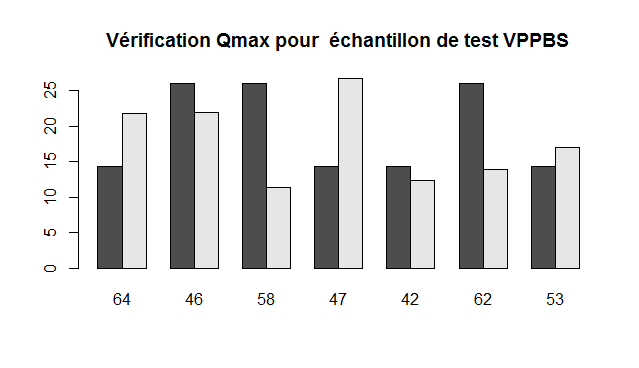
\includegraphics[width=0.75\textwidth]{../Fig/VPPBS/vppbs-regtree-test-qmax12.png}
\caption{VPPBS: Evaluation des prévisions pour Qmax à 12 mois}
\label{fig-vppbs-regtree-test-qmax12}
\end{figure}

